
\section{Overview of the FAIR facility}
The Facility of Antiproton and Ion Research in Europe (\gls{FAIR})~\cite{Spiller_2020} is an international initiative which aims to create a research facility for accelerator based research. 
\begin{figure}[!h]
    \centering
    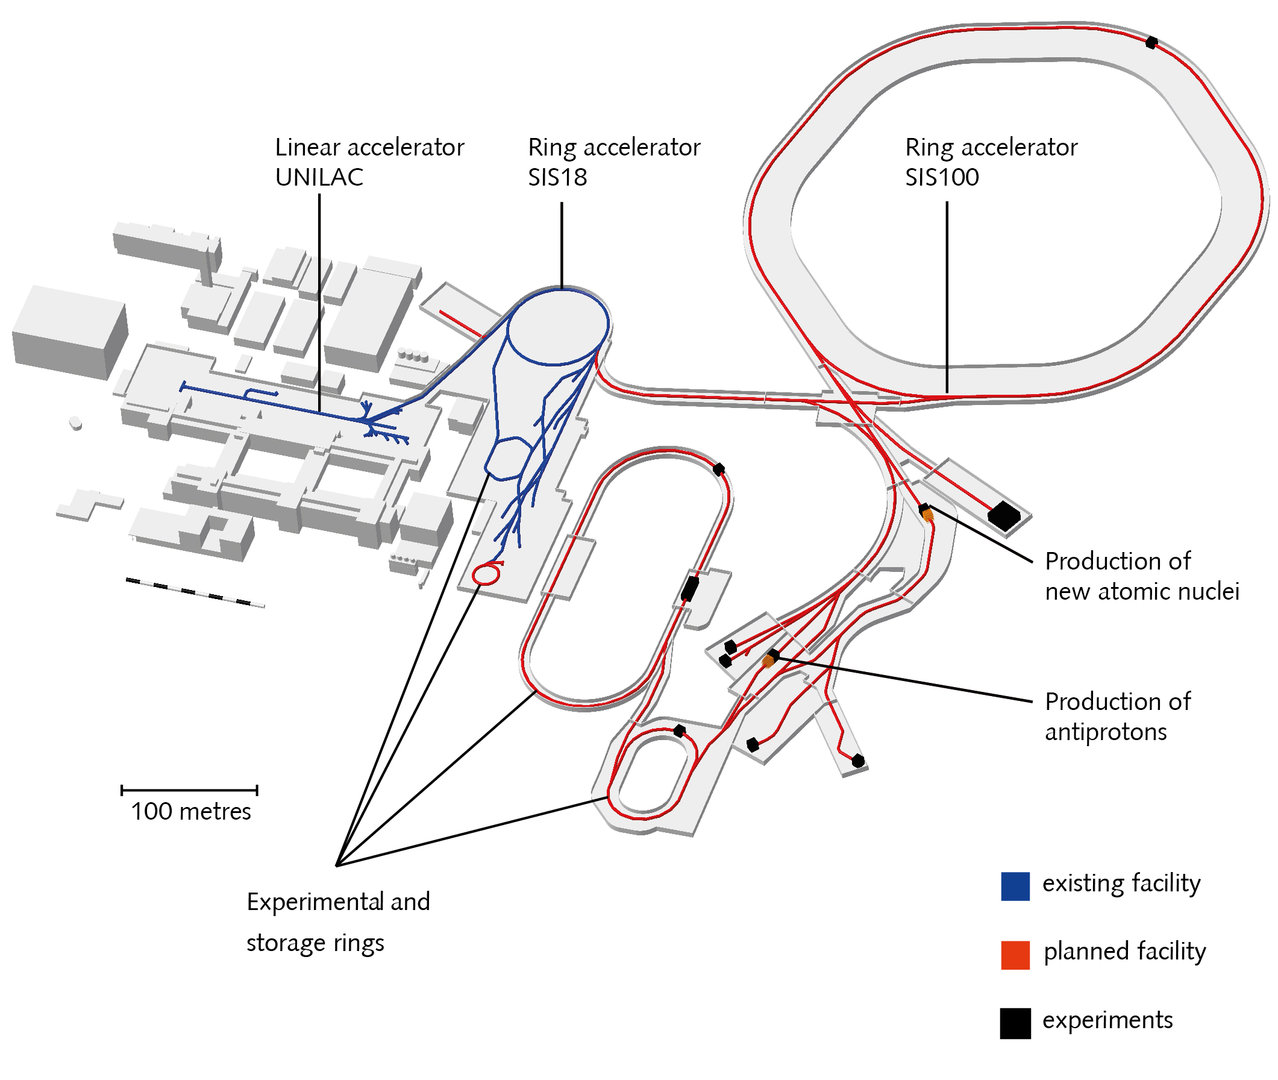
\includegraphics[width=0.65\columnwidth]{Chapter2/images/fair.jpg}
    \caption{Overview of the GSI/FAIR research facility~\cite{fair}}
    \label{fig:fair}
\end{figure}
It will provide unique research opportunities in hadron and nuclear physics, in atomic physics and nuclear astrophysics, in materials research, plasma physics and radiation biophysics, including developments of novel medical treatments and applications for space science. 
 
FAIR (see Figure \ref{fig:fair}) will extend GSI with a more capable accelerator (SIS100), storage rings and dedicated experiments from different fields, namely Atomic Physics,
Plasma physics and Applications (APPA), antiProton ANnihilation at DArmstadt
(PANDA), Nuclear Structure, Astrophysics and Reactions (NUSTAR), and Compressed Baryonic Matter (\gls{CBM}). The Schwerionensynchrotron 100 (SIS100) is
the accelerator ring built for FAIR and its experiments. The status of SIS100 and its plans were recently described by Spiller~\cite{Spiller_2020}.


The SIS100, which will provide high-intensity beams of protons up
to an energy of 29 GeV and nuclei up to 15 A GeV for Z/A = 0.5. Gold or Uranium beams will be available with kinetic energies up to 11 A GeV. High intensity secondary beams will be produced by a large acceptance Superconducting Fragment Separator, which collects very efficiently rare isotopes created in reactions with the primary beams. 